\documentclass[12pt]{kiarticle} % You can learn about my document class "kiarticle" and install it to your device by following the link: https://github.com/Kiarendil/toolkitex
\graphicspath{{pictures/}}
\DeclareGraphicsExtensions{.pdf,.png,.jpg,.eps}
%%%
\pagestyle{fancy}
\fancyhf{}
%\renewcommand{\headrulewidth}{ 0.1mm }
\renewcommand{\footrulewidth}{ .0em }
\fancyfoot[C]{\texttt{\textemdash~\thepage~\textemdash}}
\fancyhead[L]{Лабораторная работа №1.1 \hfil}
\fancyhead[R]{\hfil Иванов Кирилл, 625 группа }
\usepackage{multirow} % Слияние строк в таблице
\newcommand
{\un}[1]
{\ensuremath{\text{#1}}}
\newcommand{\eds}{\ensuremath{ \mathscr{E}}}
\newcommand{\ga}{\ensuremath{\gamma}}
\usepackage{tikz}
%%% Работа с таблицами
\usepackage{array,tabularx,tabulary,booktabs} % Дополнительная работа с таблицами
\usepackage{longtable}  % Длинные таблицы
\usepackage{multirow} % Слияние строк в таблице

\begin{document}
	
	\begin{titlepage}
		\begin{center}
			\large 	Московский физико-технический институт \\
			(государственный университет) \\
			Факультет общей и прикладной физики \\
			\vspace{0.2cm}
			
			\vspace{4.5cm}
			Лабораторная работа № 1.1  \\ \vspace{0.2cm}
			\large (Общая физика: квантовая физика) \\ \vspace{0.2cm}
			\LARGE \textbf{ Экспериментальная проверка уравнения Эйнштейна
				для фотоэффекта и определение постоянной Планка }
		\end{center}
		\vspace{2.3cm} \large
		
		\begin{center}
			Работу выполнил: \\
			Иванов Кирилл,
			625 группа
			\vspace{10mm}		
			
		\end{center}
		
		\begin{center} \vspace{60mm}
			г. Долгопрудный \\
			2018 год
		\end{center}
	\end{titlepage}


	\paragraph*{Цель работы:} 
	Исследовать зависимость фототока от величины задерживающего потенциала и частоты падающего излучения, что позволяет вычислить величину постоянной Планка.
	
	\section{Теоретическое введение}
	
	Фотоэффект --- явление испускания электронов фотокатодом, облучаемым светом,  Это явление хорошо объясняется фотонной теорией света. Взаимодействие монохроматического света с веществом можно описывать
	как взаимодействие с веществом частиц, называемых фотонами, которые обладают энергией $ \hbar \omega $ и импульсом $ \hbar\omega/c $. При столкновении фотона с электроном фотокатода энергия отона полностью передается электрону, и фотон прекращает свое существование. Энергетический баланс этого взаимодействия для вылетающих электронов
	описывается уравнением
	
	\begin{equation}\label{energy balance}
	\hbar \omega = E_{max} + W
	\end{equation}
	
	\begin{wrapfigure}{l}{0.3\linewidth}
		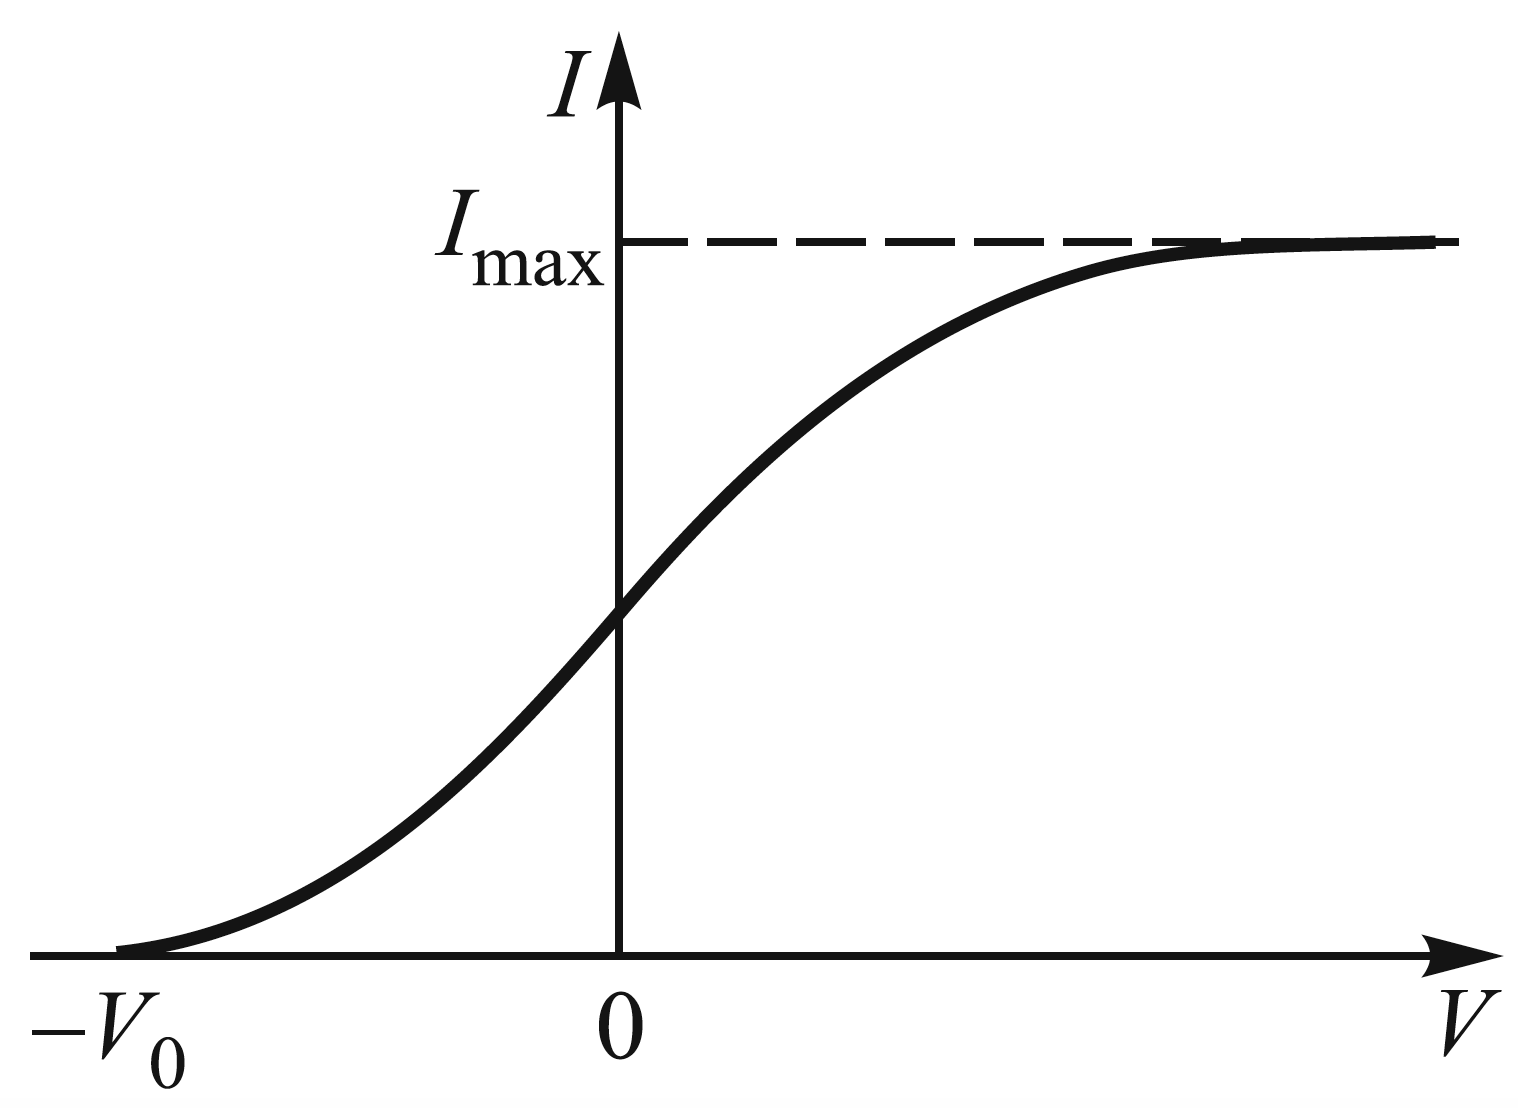
\includegraphics[width=\linewidth]{I(V)}
		\caption{Зависимость фототока от напряжения на аноде фотоэлемента}
		\label{ris I(V)}
	\end{wrapfigure}
	
	Здесь $ E_{max} $ ---  максимальная кинетическая энергия электрона после выхода из фотокатода, $ W $ --- работа выхода электрона из катода. Реально энергетический спектр вылетевших из фотокатода электронов непрерывен --- он простирается от нуля до $ E_{max} $. 
	
	Для измерения энергии вылетевших фотоэлектронов вблизи фотокатода
	обычно располагается второй электрод
	(анод), на который подается задерживающий ($ V < 0 $) или ускоряющий ($ V >
	0 $) потенциал. При достаточно больших
	ускоряющих напряжениях фототок достигает насыщения (рис. \ref{ris I(V)}): все испущенные электроны попадают на анод.
	
	При задерживающих потенциалах на анод попадают лишь электроны,
	обладающие достаточно большой кинетической энергией, в то время
	как медленно движущиеся электроны заворачиваются полем и возвращаются на катод. При некотором значении $ V = -V_0 $ (потенциал запирания) даже наиболее быстрые фотоэлектроны не могут достичь
	анода.
	Максимальная кинетическая энергия $ E_{max} $ электронов связана с
	запирающим потенциалом $ V_0 $ очевидным соотношением $ E_{max} = eV_0 $. Тогда \eqref{energy balance} примет вид, называемый уравнением Эйнштейна:
	
	\begin{equation}\label{Einsteain}
	eV_0 = \hbar\omega - W 
	\end{equation}
	
	Чтобы определить величину запирающего
	напряжения, нам надо правильно экстраполировать получаемую токовую зависимость к нулю, т. е. определить, какова функциональная
	зависимость $ I(V) $. Расчет для простейшей геометрии --- плоский катод, освещаемый светом, и параллельный ему анод --- приводит к зависимости
	
	\begin{equation}\label{sqrt I = V}
	\sqrt{I} \propto V_0 - V
	\end{equation}
	
	т. е. корень квадратный из фототока линейно
	зависит от запирающего напряжения. Эта зависимость хорошо описывает экспериментальные данные.
	
	В работе изучается зависимость фототока из фотоэлемента от величины задерживающего потенциала $ V $ для различных частот света $ \omega $, лежащих в видимой области спектра. С целью экспериментальной
	проверки уравнения Эйнштейна определяются потенциалы запирания
	$ V_0 $ при разных частотах света и строится зависимость $ V_0(\omega) $, которая, как это следует из \eqref{Einsteain}, должна иметь вид
	
	\begin{equation}\label{V(w)}
	V_0 (\omega) = \dfrac{\hbar\omega - W}{e}
	\end{equation}
	
		\begin{wrapfigure}{r}{0.3\linewidth}
		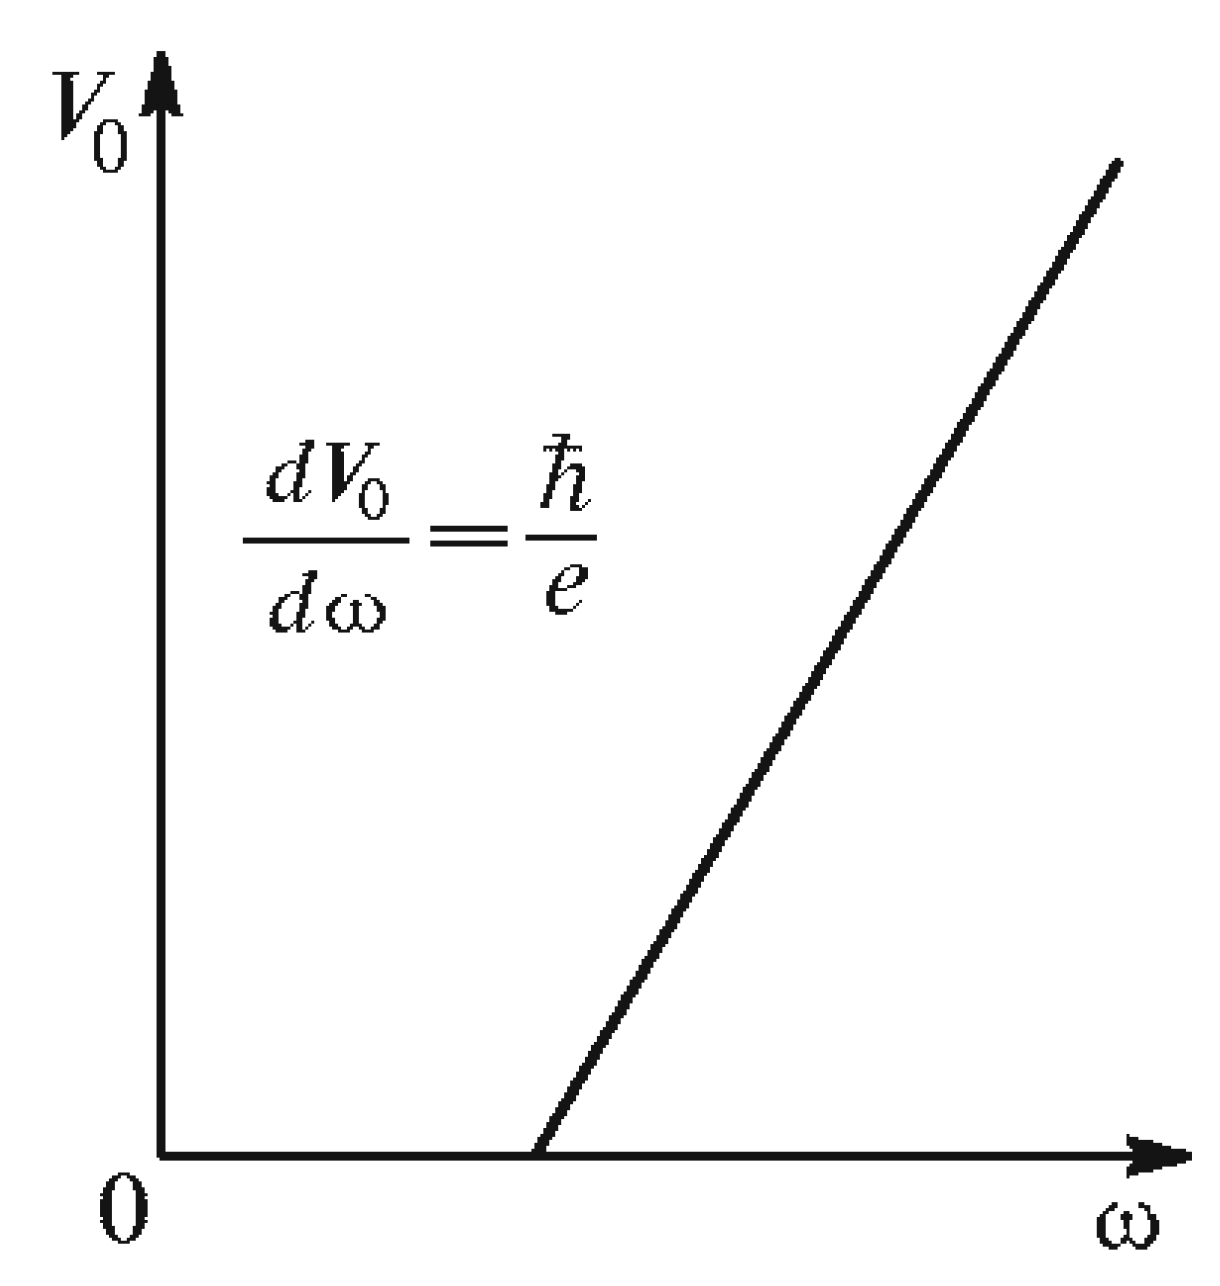
\includegraphics[width=\linewidth]{V(w)}
		\caption{Зависимость запирающего потенциала
			от частоты света}
		\label{ris V(w)}
	\end{wrapfigure}
	
	Потенциал запирания $ V_0 $ для любого катода линейно зависит от
	частоты света $ \omega $. По наклону прямой на графике $ V_0(\omega) $ (рис. \ref{ris V(w)}) можно определить постоянную Планка:
	
	\begin{equation}\label{dV/dw}
	\dfrac{dV_0}{d\omega} = \dfrac{\hbar}{e}
	\end{equation}
	
	Как показывает формула \eqref{dV/dw}, угол наклона прямой $ V_0(\omega) $ не зависит от рода вещества, из которого изготовлен фотокатод. От рода вещества, однако, зависит величина фототока, работа выхода $ W $ и форма кривой $ I(V) $ (рис. \ref{ris I(V)}). Все это определяет выбор пригодных для
	опыта катодов.


%	\section{Экспериментальная установка}
	
	
	\section{Выполнение работы}
	
	Сначала выполним градуировку монохроматора. Проведем серию измерений для линий спектра неона, снимая зависимость длины волны света от параметра $ \theta $ барабана монохроматора. Результаты занесем в таблицу и построим график зависимости, профитировав функцию $ \lambda (\theta) $ многочленом второй степени в силу нелинейности. 
	
		\begin{table}[h!]
		\caption{Градуировка монохроматора}
		\begin{center}
			\begin{tabular}{|c|c|c|}
				\hline 
				№  линии & $ \theta $, $ ^\circ $ & $ \lambda, \;\mathring{A} $   \\ 
				\hline 
			23 & 1872 & 5400 \\
			22 & 2130 & 5828 \\
			21 & 2146 & 5885 \\
			20 & 2174 & 5944 \\
			19 & 2192 & 5975 \\
			18 & 2218 & 6030 \\
			17 & 2235 & 6074 \\
			16 & 2248 & 6096 \\
			15 & 2266 & 6143 \\
			14 & 2274 & 6163 \\
			13 & 2298 & 6217 \\
			12 & 2318 & 6266 \\
			11 & 2334 & 6304 \\
			10 & 2346 & 6334 \\
			9 & 2363 & 6382 \\
			8 & 2372 & 6402 \\
			7 & 2412 & 6506 \\
			6 & 2418 & 6532 \\
			5 & 2440 & 6598 \\
			4 & 2466 & 6678 \\
			3 & 2478 & 6717 \\
			2 & 2544 & 6929 \\
			1 & 2575 & 7032 \\
				\hline 
			\end{tabular} 
		\end{center}
		\label{table g}
	\end{table}

\begin{figure}[h!]
	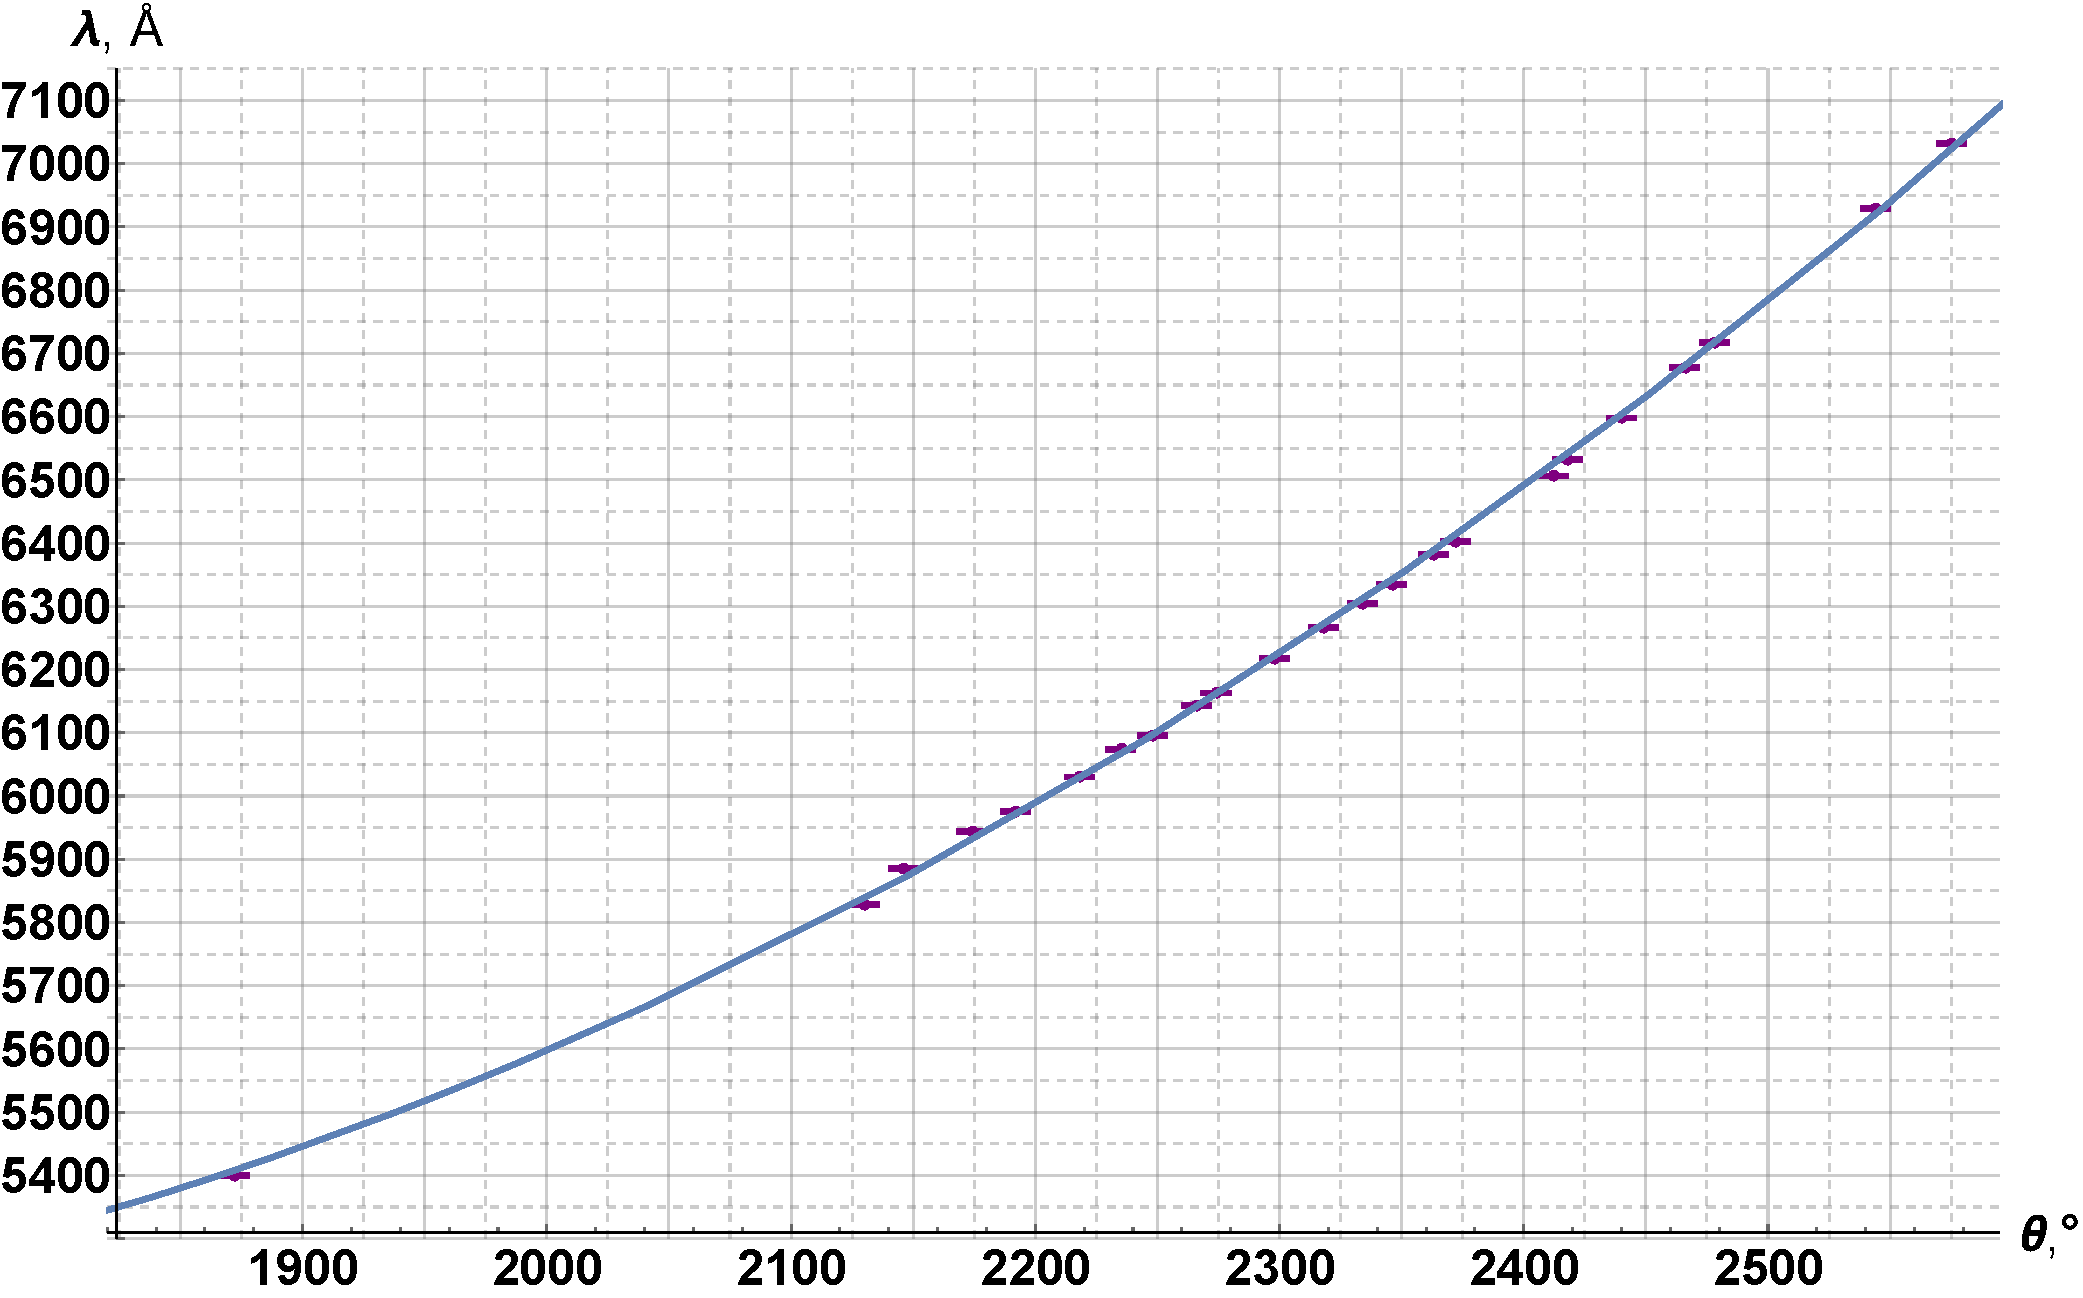
\includegraphics[scale=0.5]{G.pdf}
	\caption{Градуировка монохроматора}
	\label{graf_g}
\end{figure} 

	\begin{table}[H]
	\caption{Фит рис. \ref{graf_g} функцией $ y = ax^2 + bx + c $}
	\begin{center}
		\begin{tabular}{|c|c|c|}
			\hline
			& \text{Estimate} & \text{Standard Error} \\
			\hline
			 $ c $ & 7931.34 & 249.707 \\
			$ b $ & -3.99555 & 0.221236 \\
			$ a $ & 0.00141429 & 0.0000489127 \\
			\hline 
		\end{tabular} 
	\end{center}
	\label{}
\end{table}
	
	Теперь проведем 5 серий измерений зависимости фототока от напряжения для разных длин волн падающего света, изменяя на монохроматоре параметр $ \theta $ и переводя его в длину волны с помощью градуировки. Ток приведен в безразмерных единицах в силу работы установки. 
	
	Результаты измерений сведем в таблицы. Для первой выбранной длины волны ($ \theta = 2174^\circ, \lambda = 6944 \mathring{A}$) проведем измерения во всем спектре возможных напряжений, а для остальных --- лишь при достаточно малых значениях тока и напряжения (т.е. вблизи потенциала запирания, где искомая зависимость описывается формулой \eqref{sqrt I = V}). Согласно этой формуле \eqref{sqrt I = V}, построим графики зависимости в координатах $ \sqrt{I} (V) $ и аппроксимируем линейные участки прямой. Экстраполируя прямую к нулю, получим значения потенциала запирания для каждой серии измерения (длины волны). Результаты сведем в таблицу. 
	
		\begin{table}[h!]
		\caption{Зависимость фототока от напряжения для $ \theta = 2174^\circ $}
		\begin{center}
			\begin{tabular}{|c|c|c|c|}
				\hline
				 № & $ V $, В & $ I $ & $ \sqrt{I}  $ \\
				\hline
				 1. & 6.797 & 0.586 & 0.766 \\
				2. & 6.223 & 0.582 & 0.763 \\
				3. & 5.782 & 0.577 & 0.76 \\
				4. & 5.235 & 0.571 & 0.756 \\
				5. & 4.701 & 0.563 & 0.75 \\
				6. & 4.2 & 0.556 & 0.746 \\
				7. & 3.64 & 0.545 & 0.738 \\
				8. & 3.06 & 0.531 & 0.729 \\
				9. & 2.565 & 0.515 & 0.718 \\
				10. & 2.1 & 0.489 & 0.699 \\
				11. & 1.43 & 0.44 & 0.663 \\
				12. & 0.9 & 0.34 & 0.583 \\
				13. & 0.41 & 0.173 & 0.416 \\
				14. & 0.02 & 0.069 & 0.263 \\
				15. & -0.02 & 0.057 & 0.239 \\
				16. & -0.18 & 0.034 & 0.184 \\
				17. & -0.3 & 0.015 & 0.122 \\
				18. & -1.125 & -0.005 & -0.071 \\
				19. & -1.75 & -0.005 & -0.071 \\
				20. & -3.04 & -0.005 & -0.071 \\
				\hline 
			\end{tabular} 
		\end{center}
		\label{}
	\end{table}

\begin{table}[h!]
	\caption{Зависимость фототока от напряжения для разных длин волн}
	\begin{center}
		\begin{tabular}{|c|c|c|c|}
			\hline
			№ & $ V $, В & $ I $ & $ \sqrt{I}  $ \\
			\hline
			\multicolumn{4}{|c|}{Для $ \theta = 2235 $} \\
			\hline
			1. & 0.939 & 0.328 & 0.573 \\
			2. & 0.645 & 0.248 & 0.498 \\
			3. & 0.24 & 0.119 & 0.345 \\
			4. & 0.399 & 0.178 & 0.422 \\
			5. & 0.695 & 0.282 & 0.531 \\
			6. & 0.077 & 0.081 & 0.285 \\
			7. & 0.02 & 0.069 & 0.263 \\
			8. & -0.835 & 0.003 & 0.055 \\
			\hline 
			\multicolumn{4}{|c|}{Для $ \theta = 2412 $} \\
			\hline
			1. & 0.899 & 0.362 & 0.602 \\
			2. & 0.654 & 0.282 & 0.531 \\
			3. & 0.415 & 0.189 & 0.435 \\
			4. & 0.24 & 0.13 & 0.361 \\
			5. & 0.01 & 0.055 & 0.235 \\
			6. & -0.372 & 0.002 & 0.045 \\
			\hline 
			\multicolumn{4}{|c|}{Для $ \theta = 2318 $} \\
			\hline
			1. & 0.77 & 0.29 & 0.539 \\
			2. & 0.55 & 0.23 & 0.48 \\
			3. & 0.358 & 0.16 & 0.4 \\
			4. & 0.083 & 0.077 & 0.277 \\
			5. & -0.022 & 0.052 & 0.228 \\
			6. & -0.147 & 0.027 & 0.164 \\
			7. & -0.45 & 0.003 & 0.055 \\
			\hline 
			\multicolumn{4}{|c|}{Для $ \theta = 1872 $} \\
			\hline
			1. & 1.417 & 0.322 & 0.567 \\
			2. & 1.07 & 0.253 & 0.503 \\
			3. & 0.76 & 0.182 & 0.427 \\
			4. & 0.41 & 0.117 & 0.342 \\
			5. & 0.12 & 0.075 & 0.274 \\
			6. & 0. & 0.04 & 0.2 \\
			7. & -0.128 & 0.025 & 0.158 \\
			8. & -0.754 & -0.016 & -0.126 \\
			\hline
		\end{tabular} 
	\end{center}
	\label{}
\end{table}

\begin{figure}[h!]
	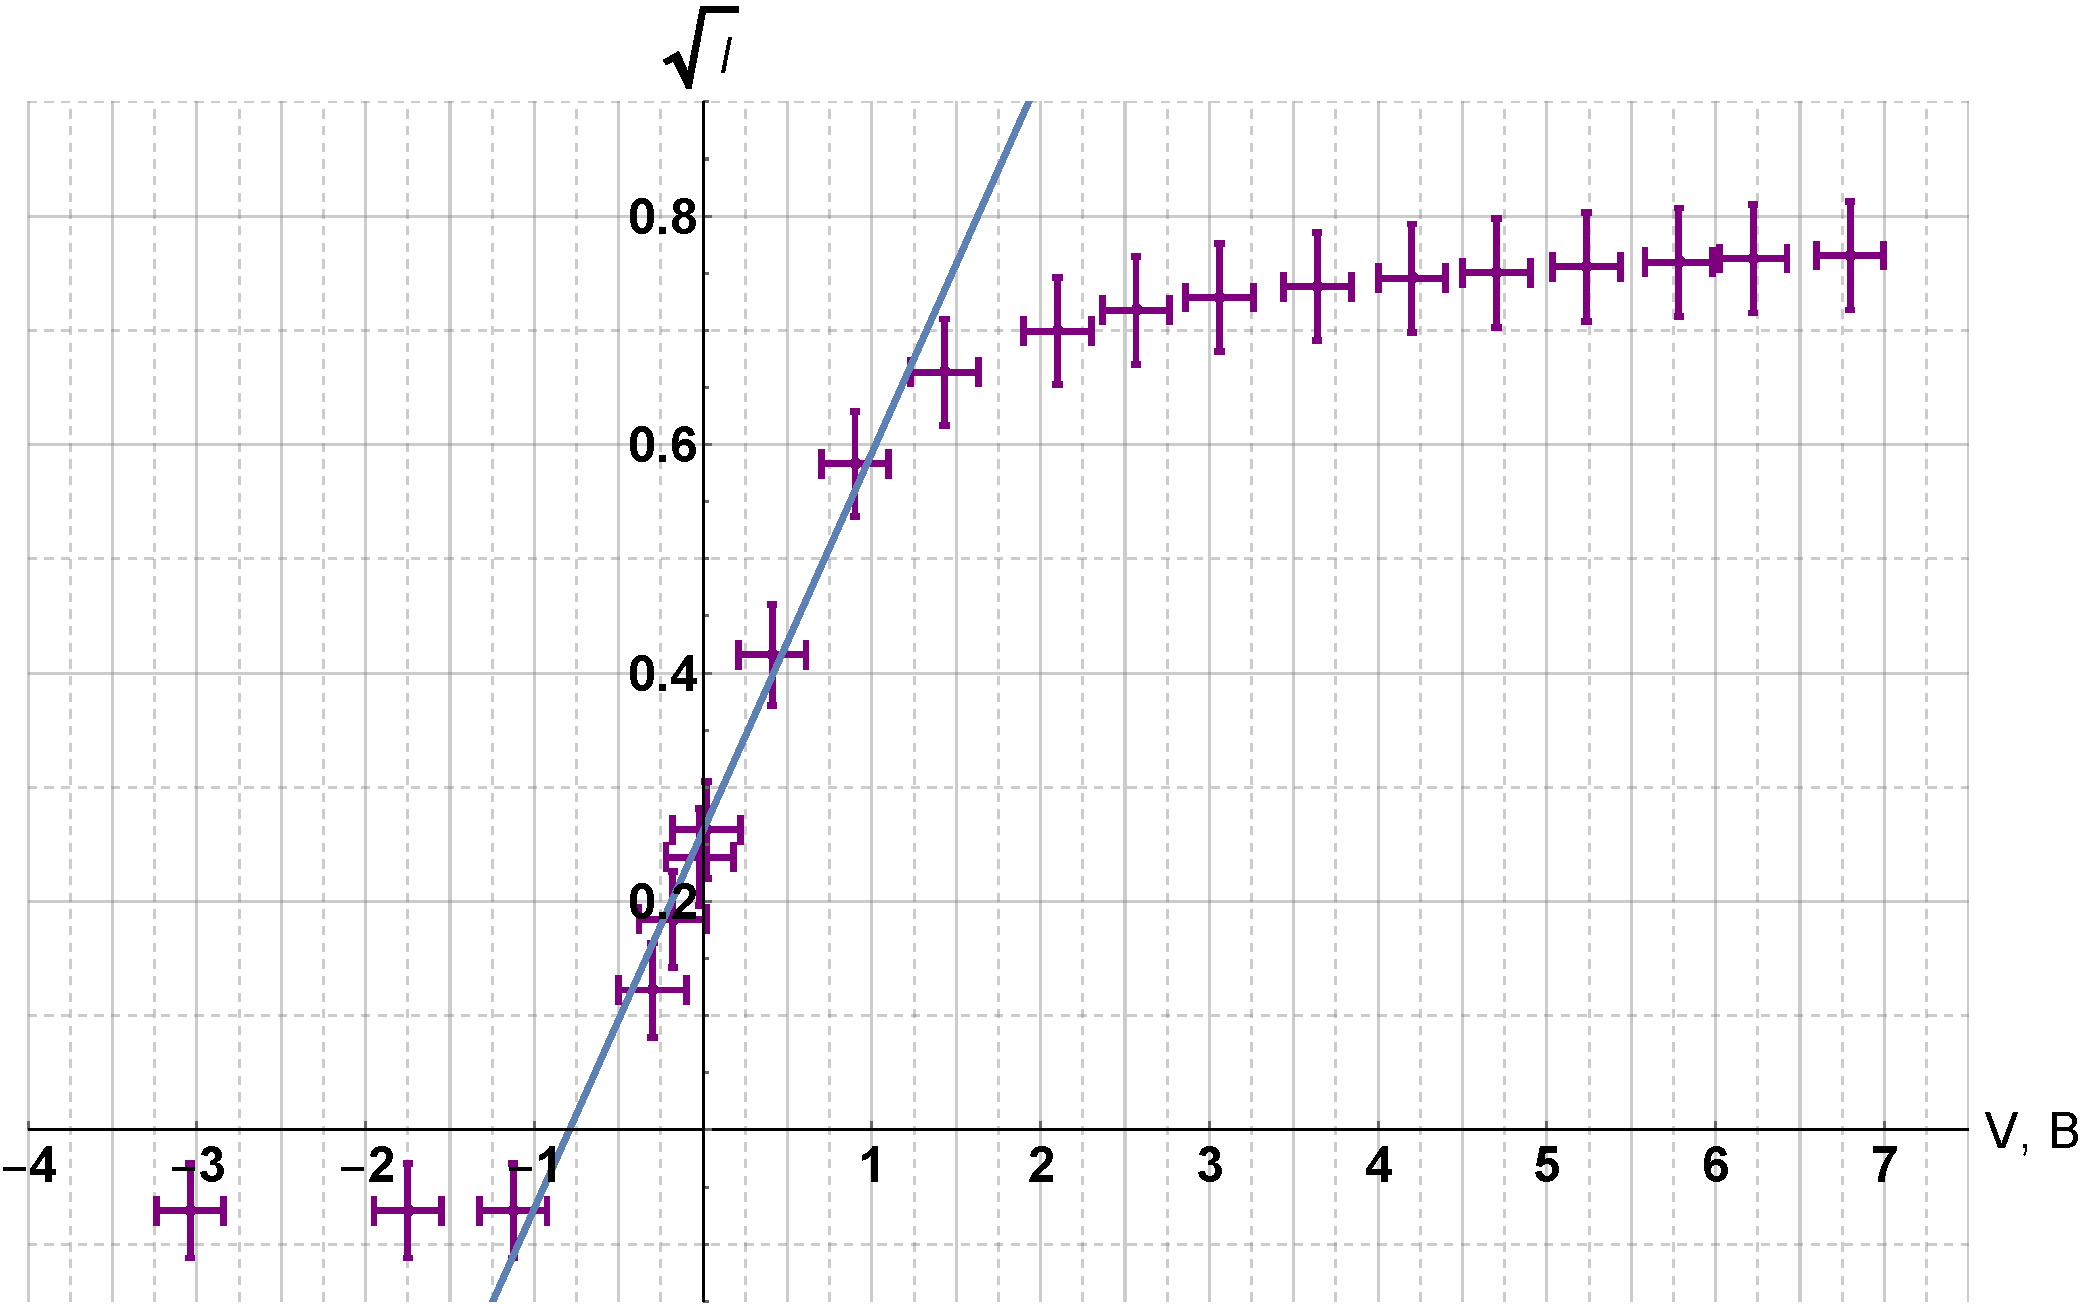
\includegraphics[scale=0.5]{Ibig.pdf}
	\caption{Зависимость фототока от напряжения для $ \theta = 2174^\circ $}
	\label{graf_Ibig}
\end{figure} 

\begin{figure}[h!]
	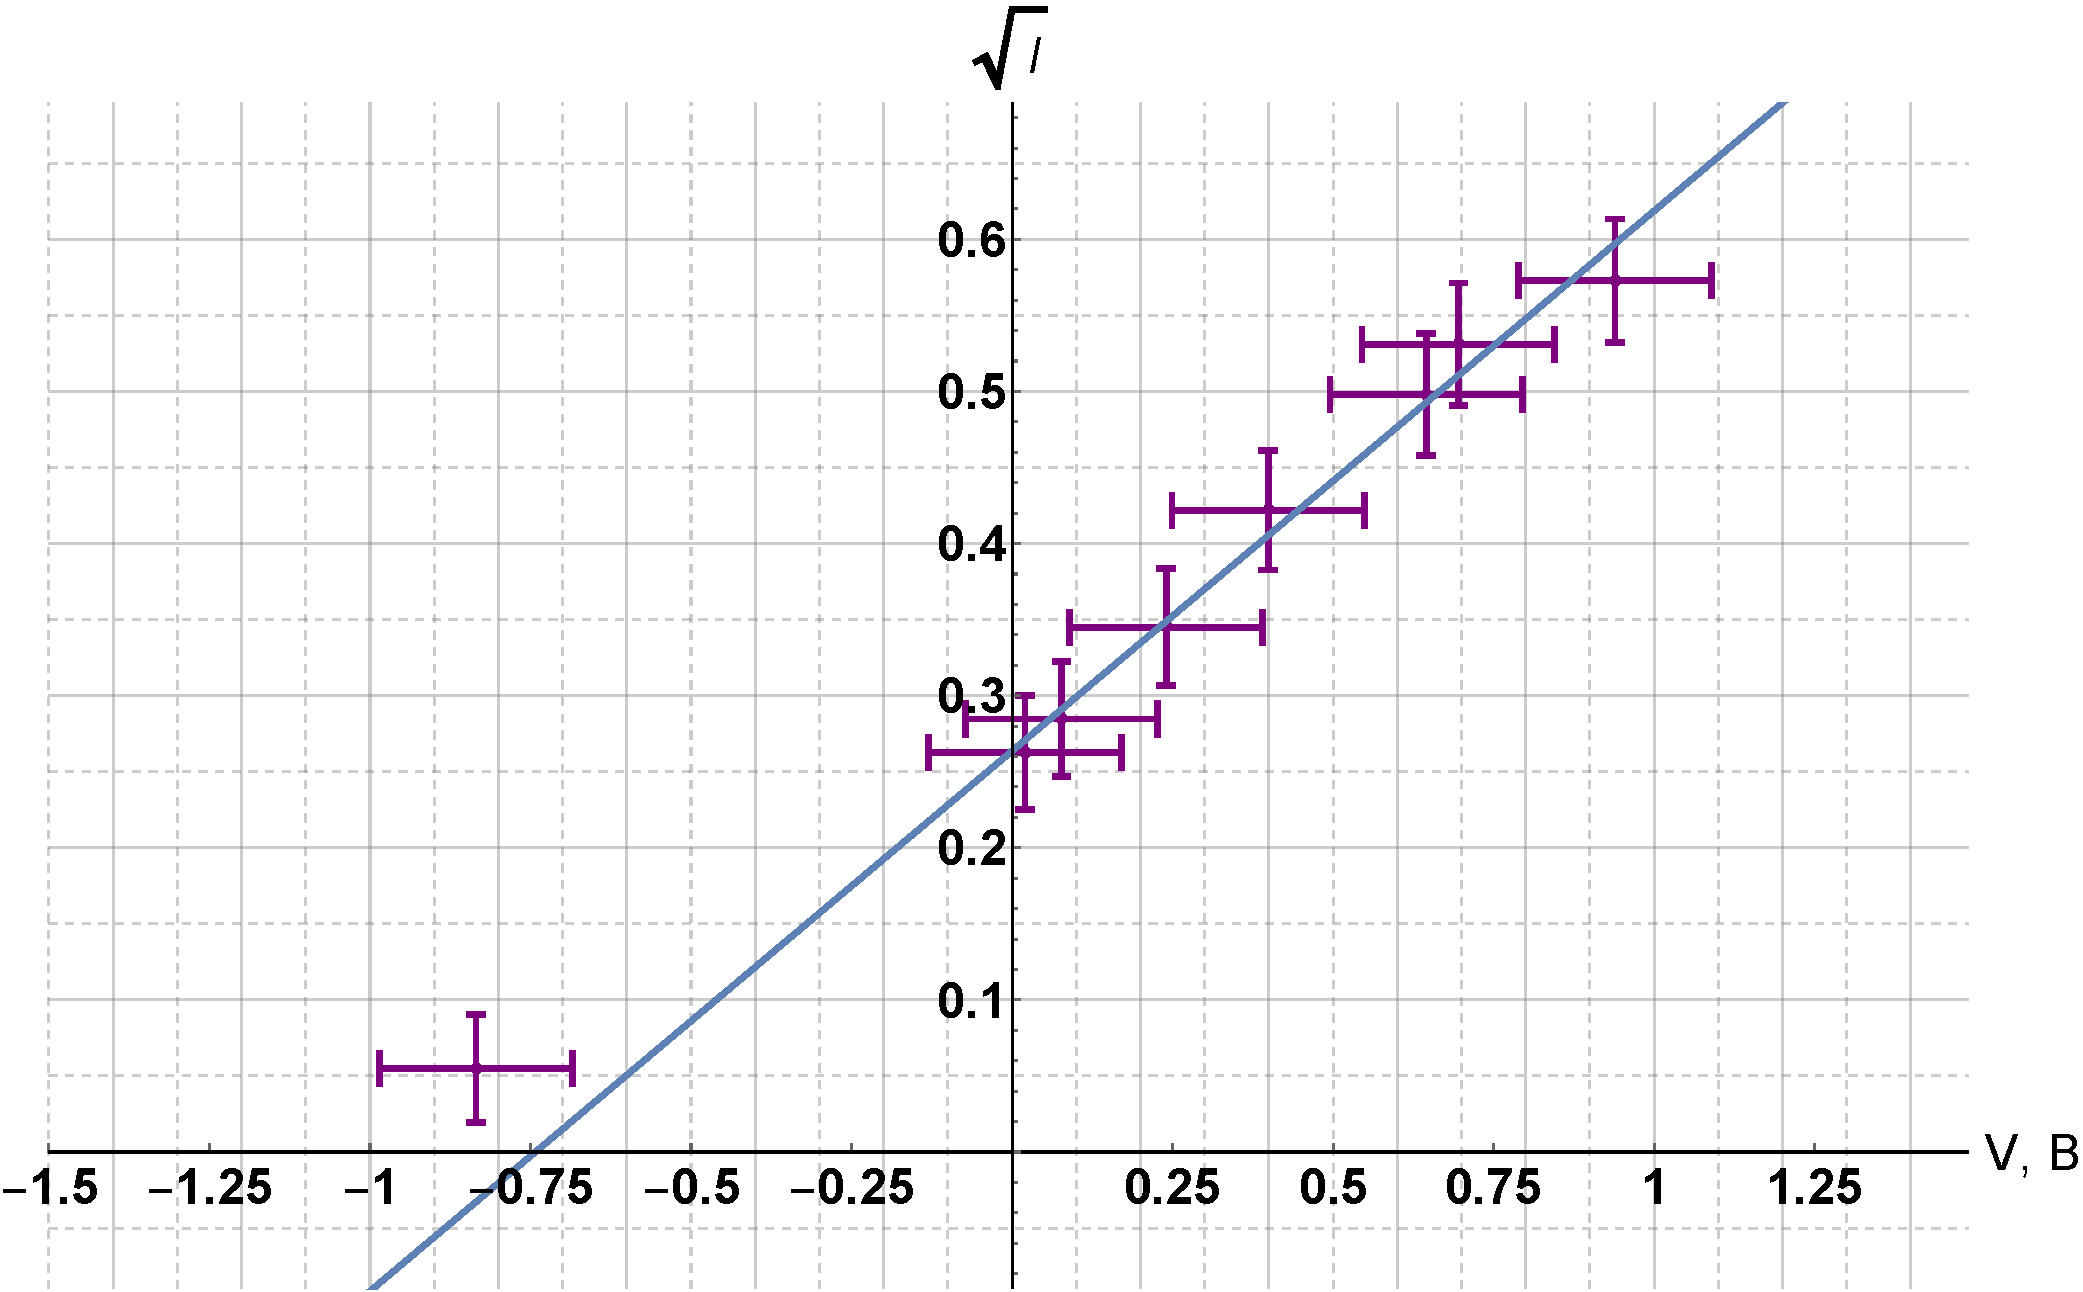
\includegraphics[scale=0.5]{2235.pdf}
	\caption{Зависимость фототока от напряжения для $ \theta = 2235^\circ $}
	\label{graf 2235}
\end{figure} 

\begin{figure}[h!]
	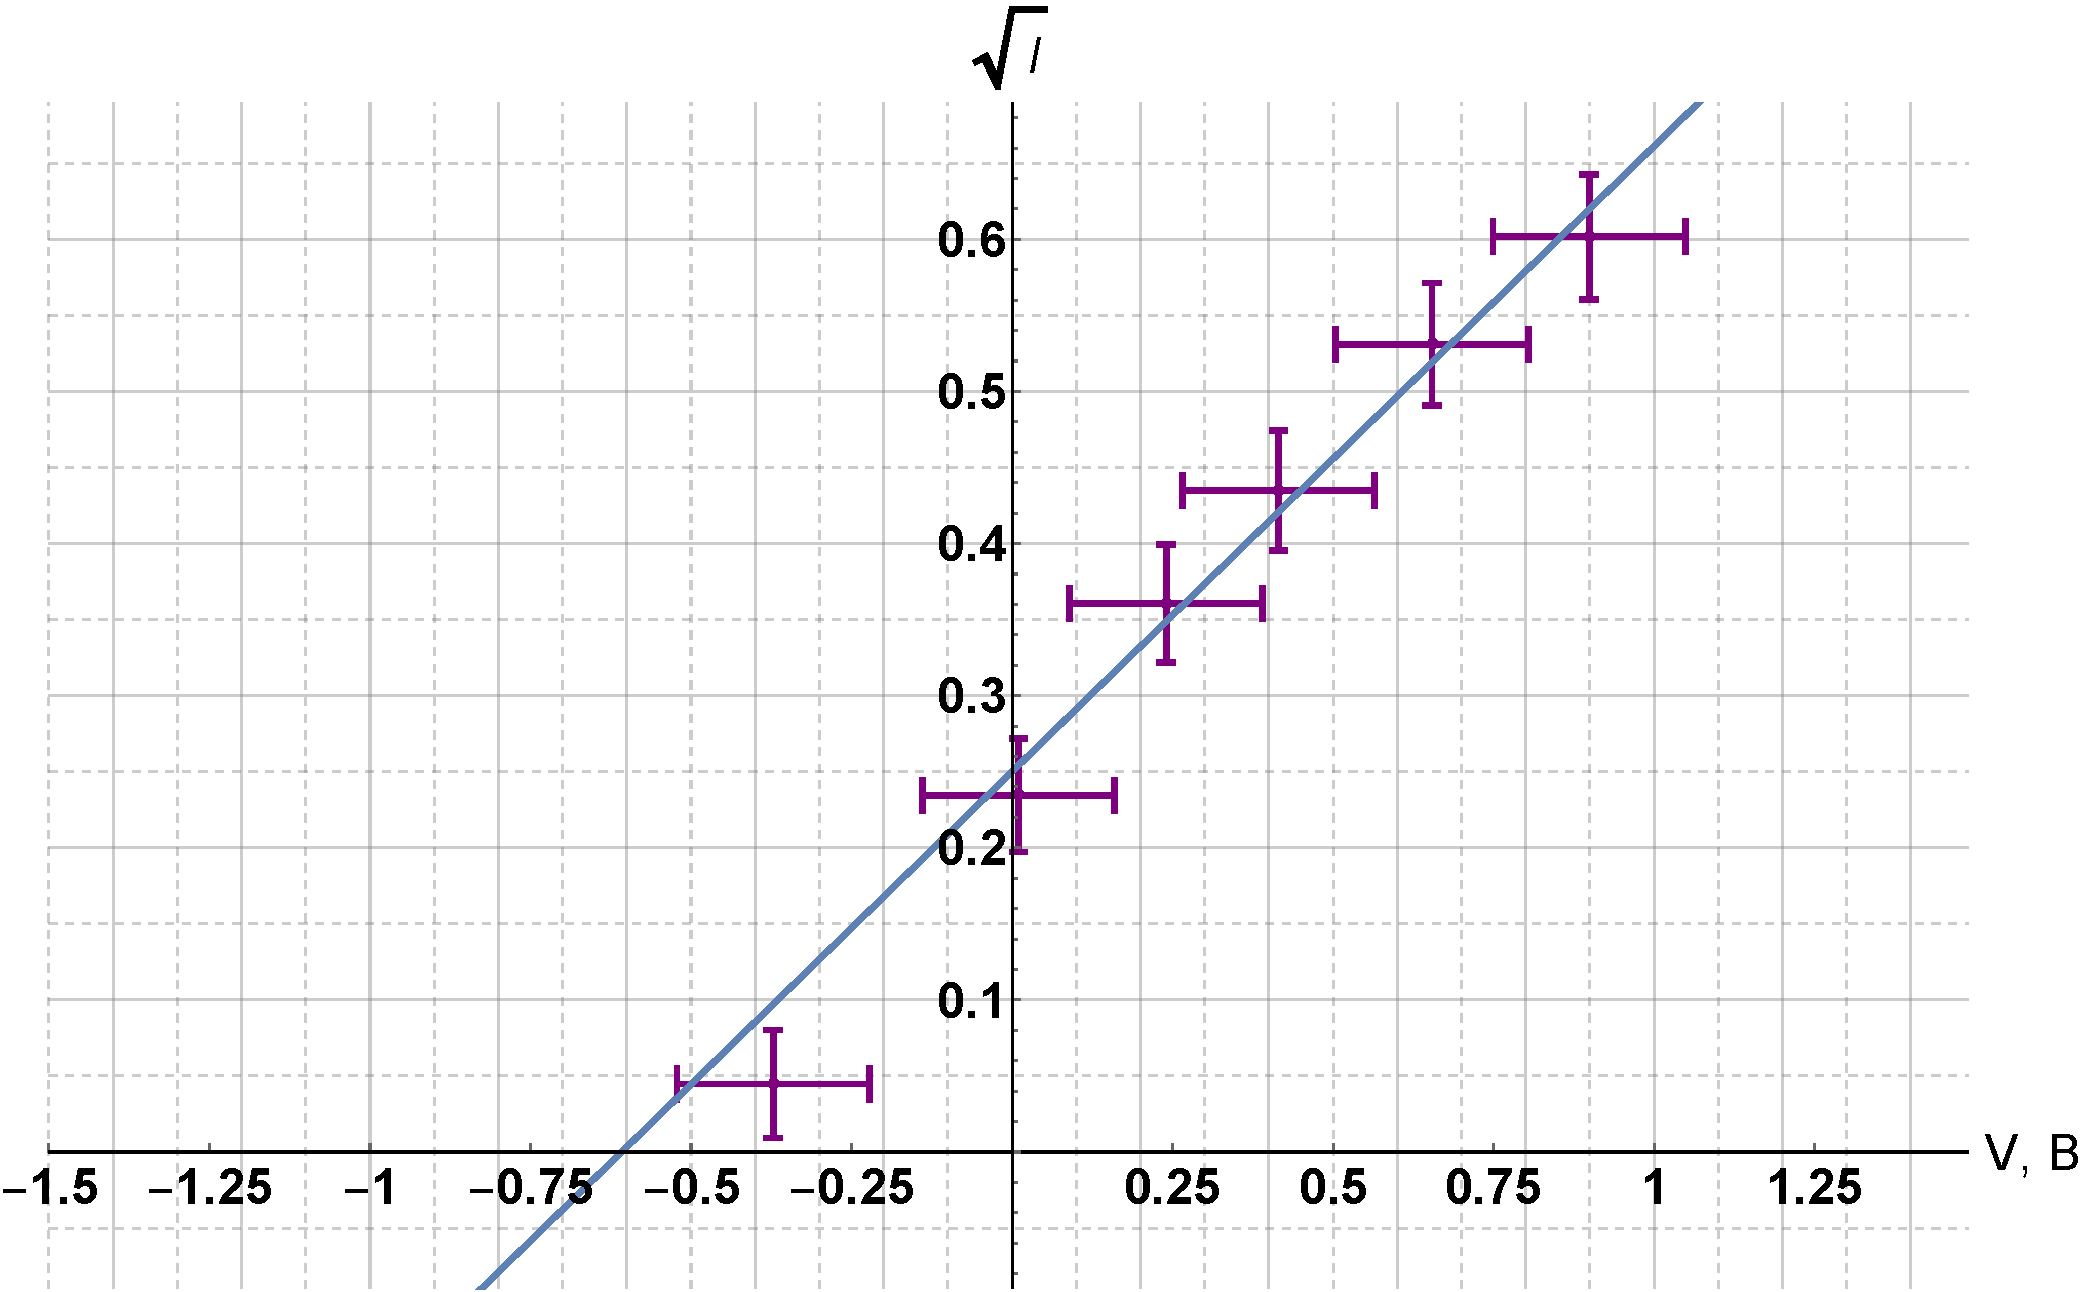
\includegraphics[scale=0.5]{2412.pdf}
	\caption{Зависимость фототока от напряжения для $ \theta = 2412^\circ $}
	\label{graf 2412}
\end{figure} 

\begin{figure}[h!]
	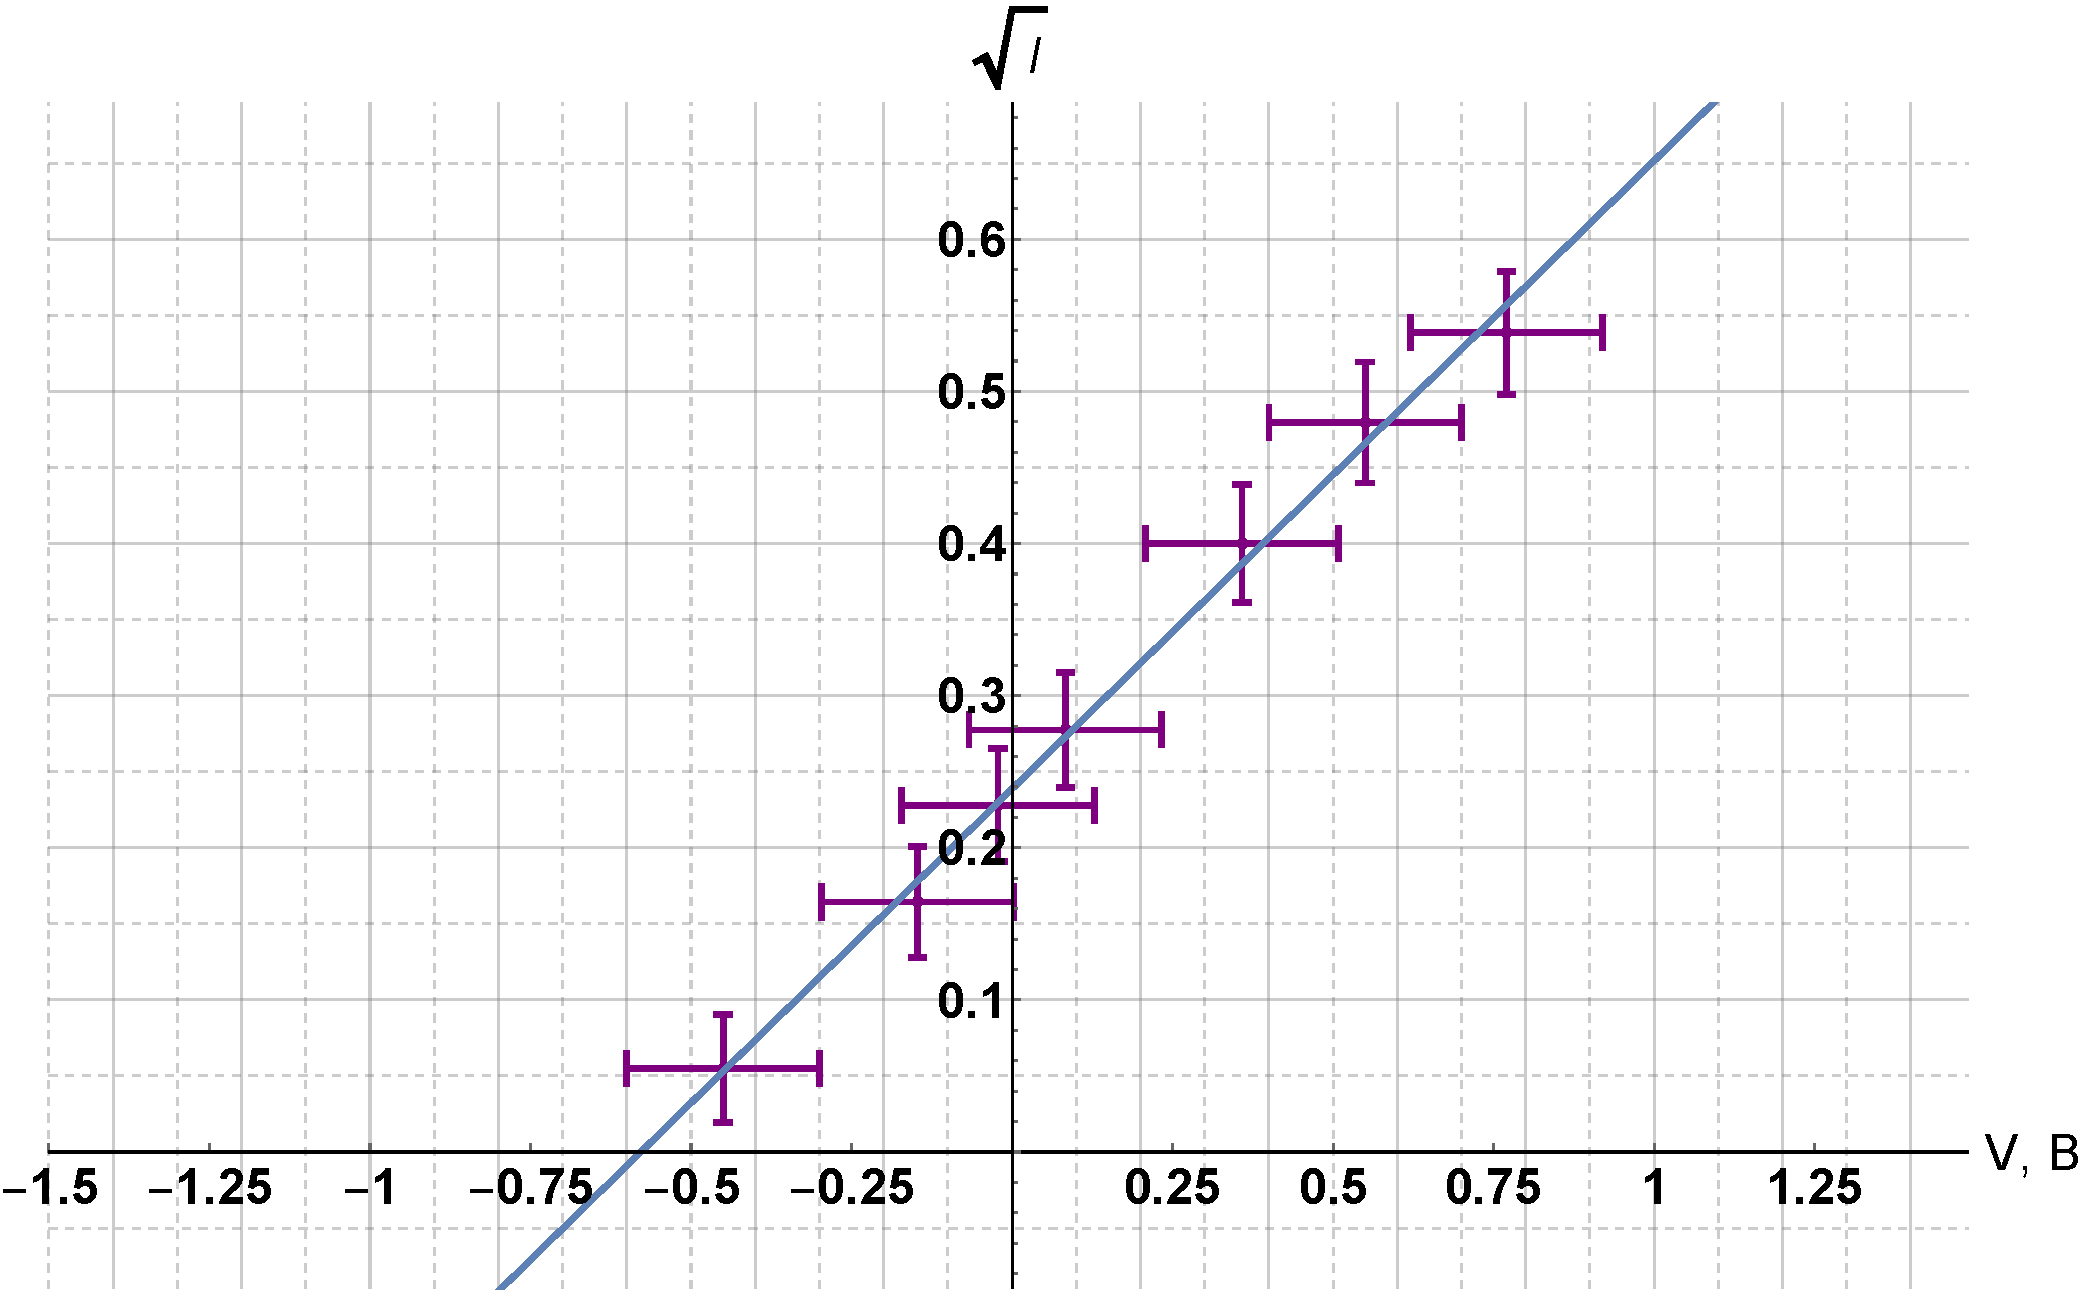
\includegraphics[scale=0.5]{2318.pdf}
	\caption{Зависимость фототока от напряжения для $ \theta = 2318^\circ $}
	\label{graf 2318}
\end{figure} 
	
	\begin{figure}[h!]
		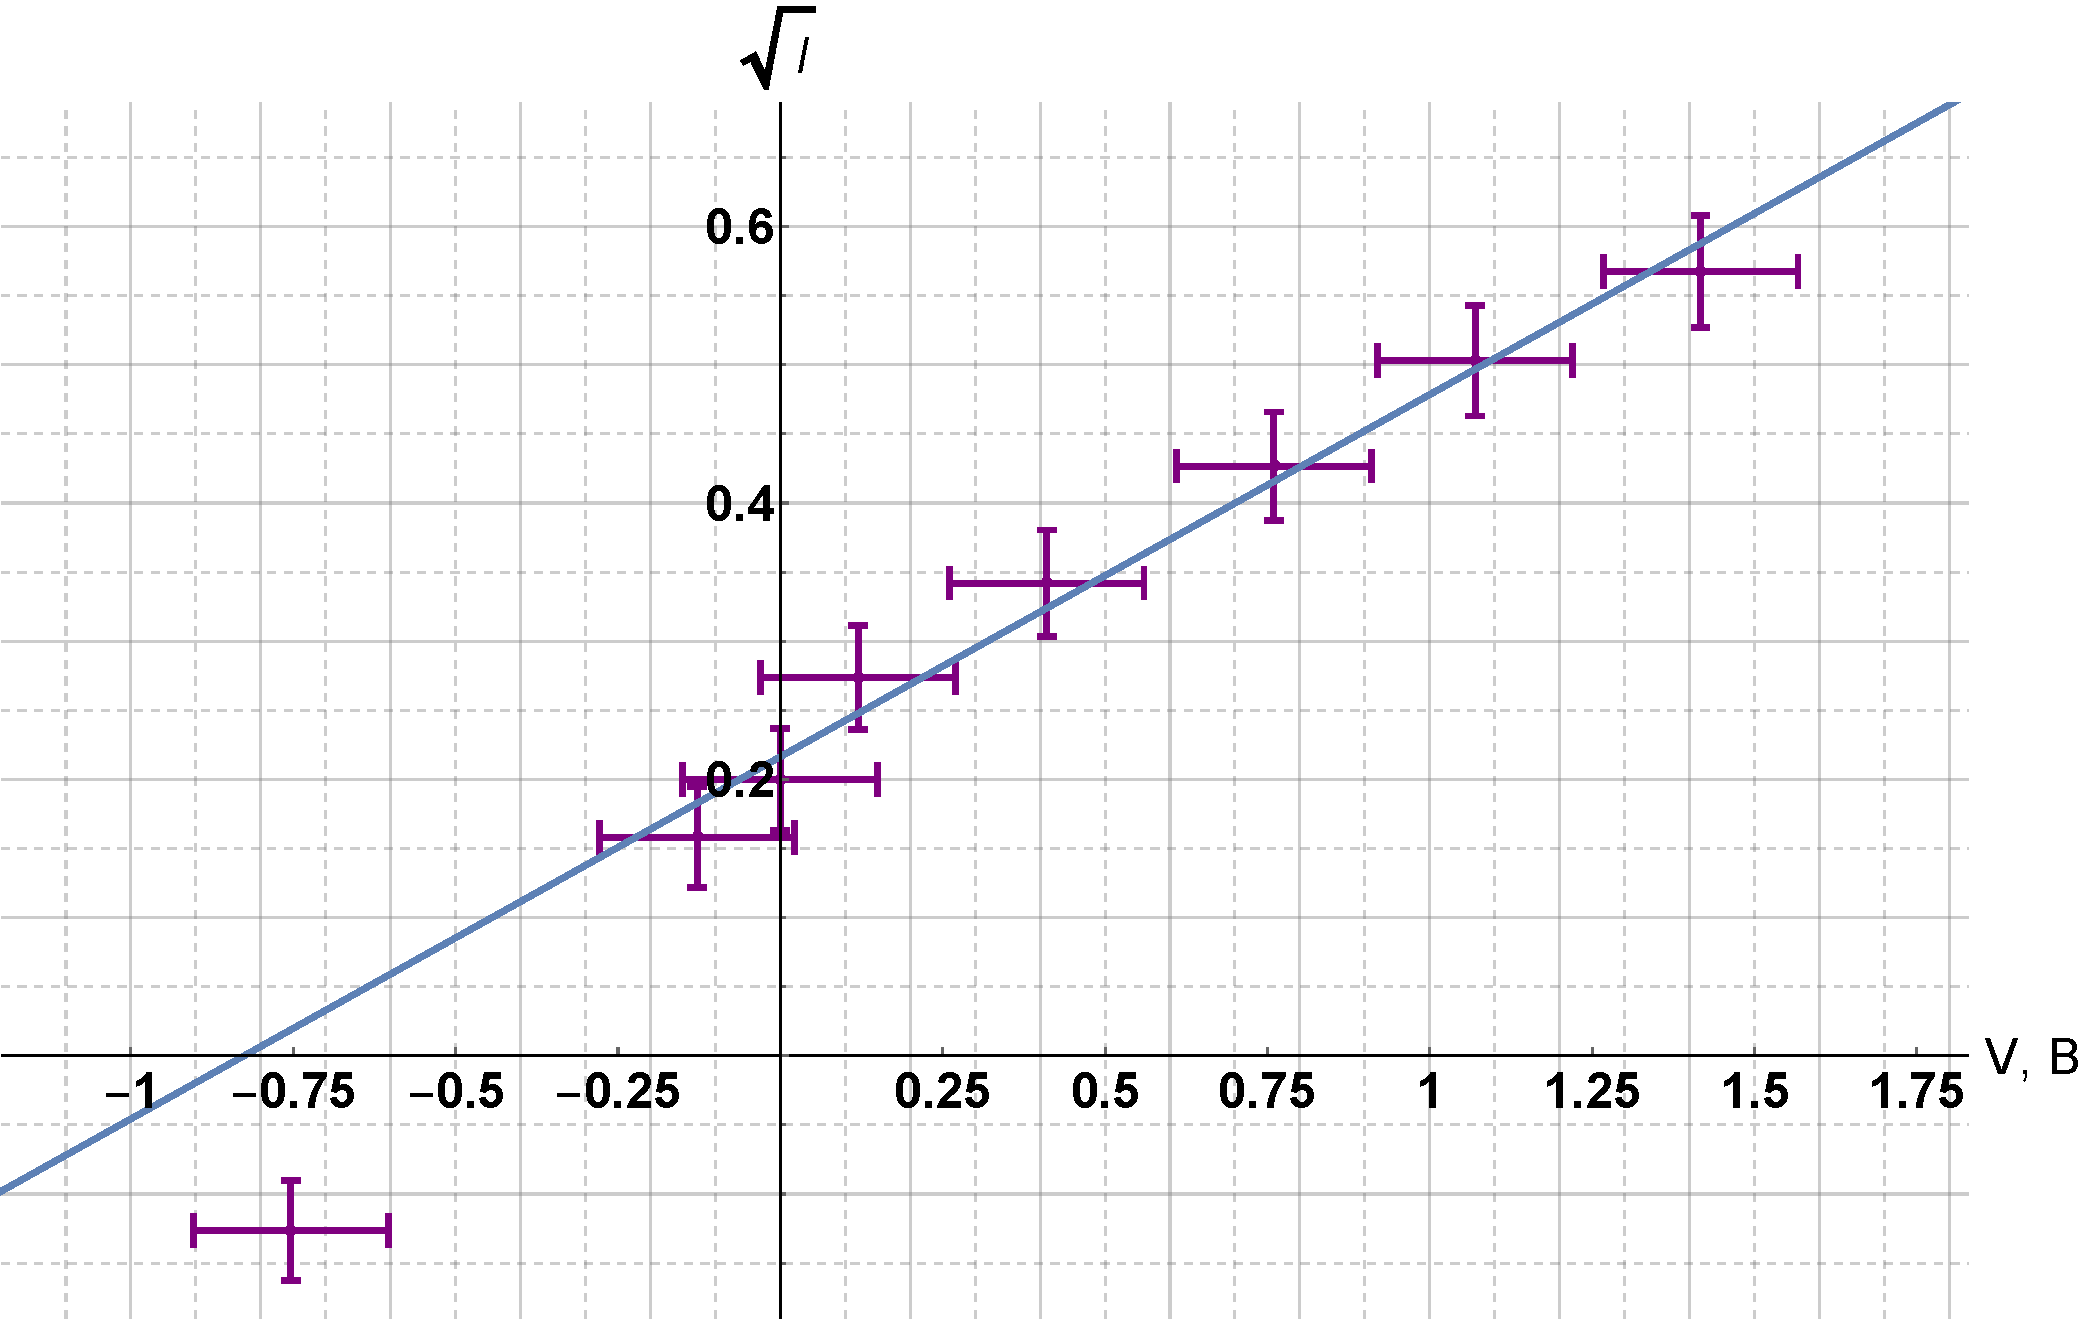
\includegraphics[scale=0.5]{1872.pdf}
		\caption{Зависимость фототока от напряжения для $ \theta = 1872^\circ $}
		\label{graf 1872}
	\end{figure} 

\begin{table}[h!]
	\caption{Результаты измерений для разных длин волн, параметры фитов для $ y = ax + b $}
	\begin{center}
		\begin{tabular}{|c|c|c|c|c|c|c|c|}
			\hline
			№ & $ \theta, \; ^\circ $& $ \lambda, \; \mathring{A} $ &  $ \omega, \; 10^{15} $ с & $ a $ & $ b $ & $ V_0 $, В & $ \sigma_{V_0} $, В \\
			\hline
		 1 & 2174 & 5944 & 3.16958 & 0.381001 $ \pm 0,0140678 $ & 0.248515 $ \pm 0,0093133 $& 0.792 & 0.059 \\
		2 & 2235 & 6074 & 3.10175 & 0.355079 $ \pm 0,0202219 $ & 0.263619 $ \pm 0,0108196 $& 0.742 & 0.056 \\
		3 & 2412 & 6506 & 2.89579 & 0.445597 $ \pm 0,0233336 $& 0.230778 $ \pm 0,0120653 $& 0.518 & 0.039 \\
		4 & 2318 & 6266 & 3.0067 & 0.412892 $ \pm 0,0170772 $ & 0.238741 $ \pm 0,00953726 $& 0.578 & 0.043 \\
		5 & 1872 & 5400 & 3.48889 & 0.262064 $ \pm0,0155836 $ & 0.216402 $ \pm 0,0116755 $& 0.826 & 0.062 \\
			\hline
		\end{tabular} 
	\end{center}
	\label{}
\end{table}
	\newpage
	.
	\begin{figure}[H]
		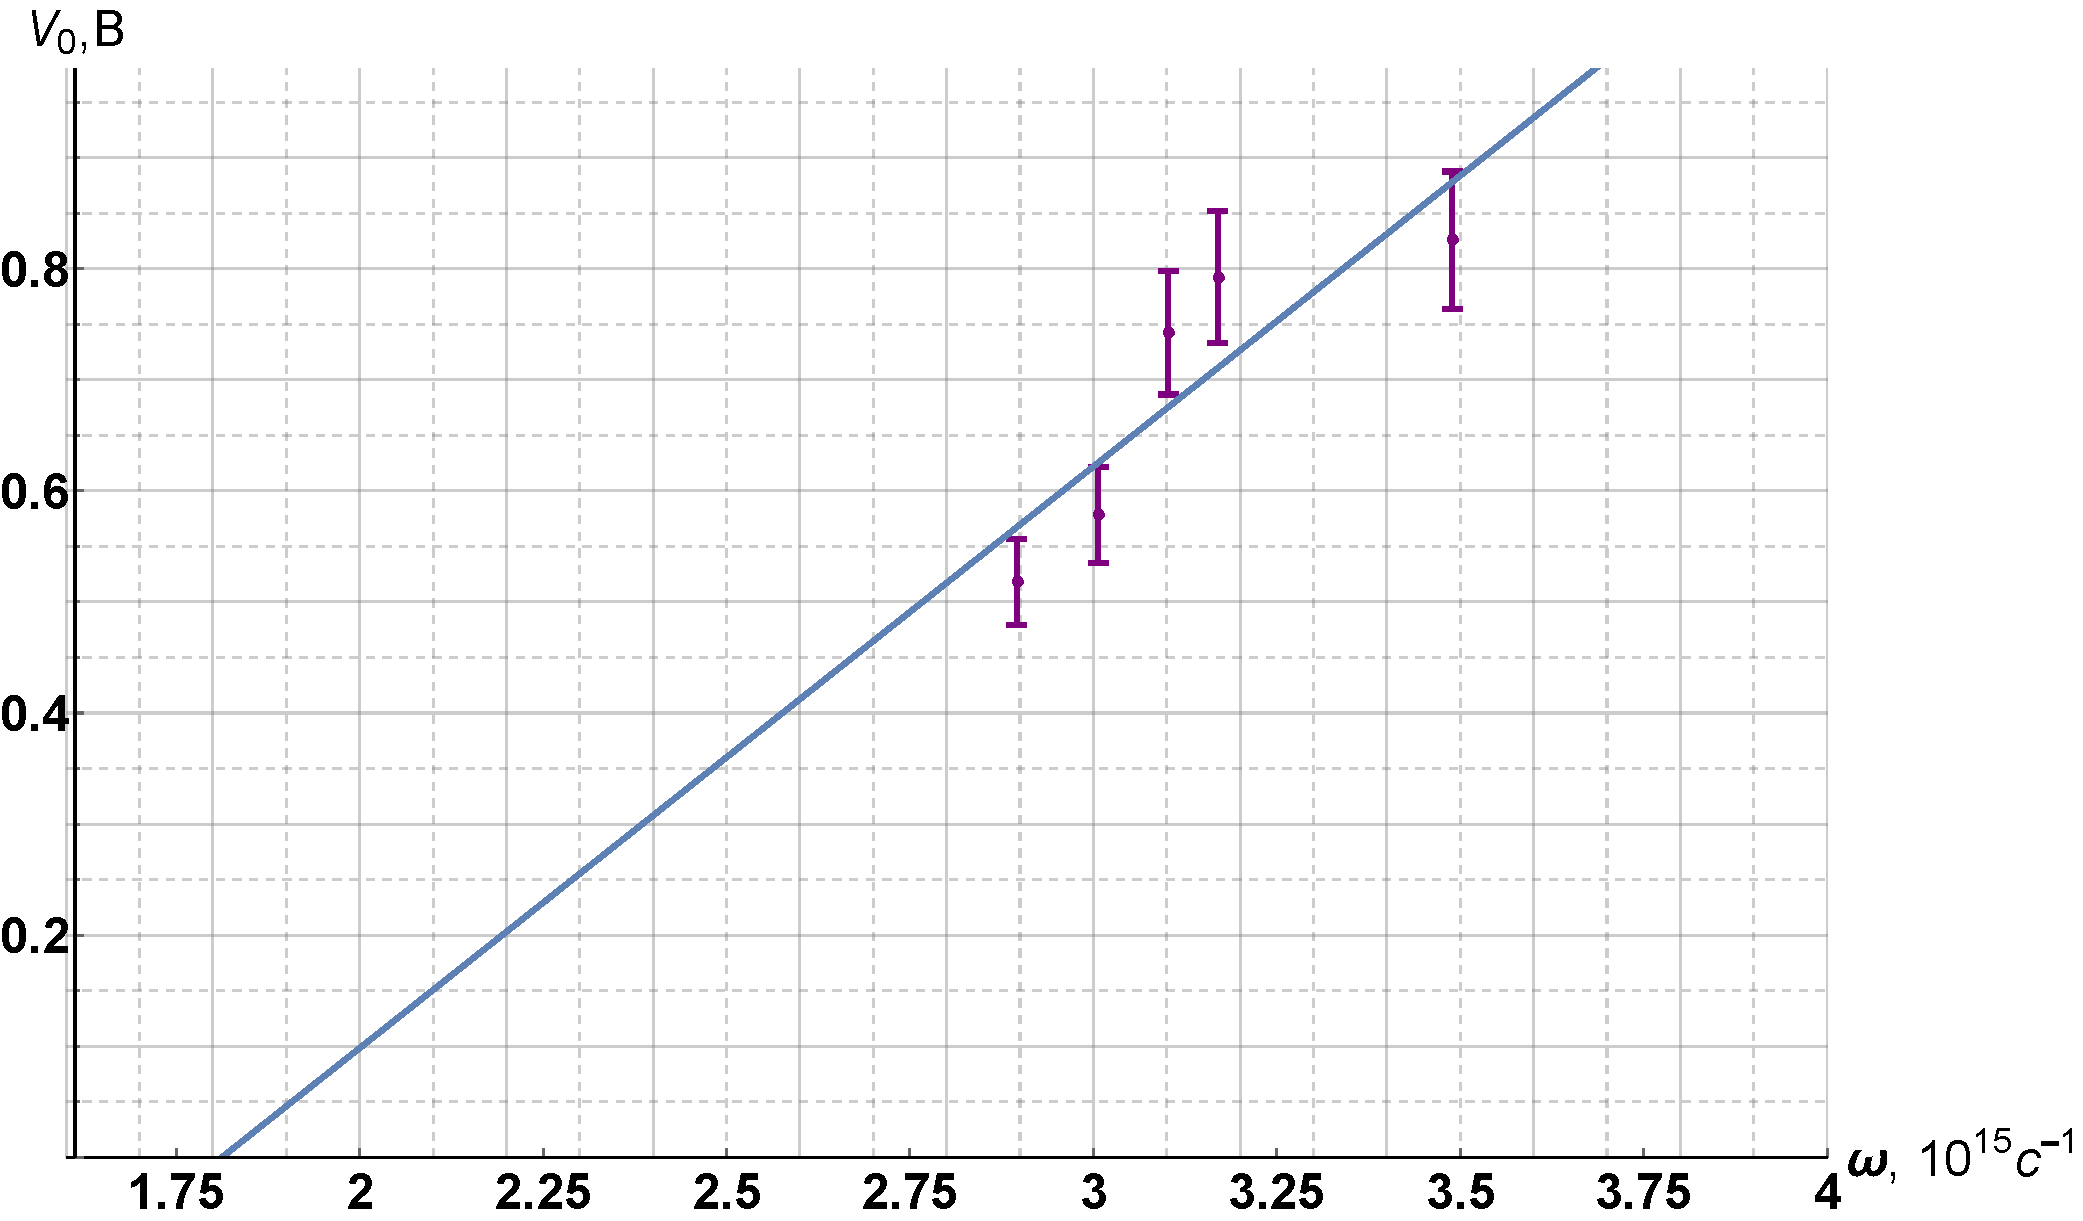
\includegraphics[scale=0.5]{V0.pdf}
		\caption{Зависимость запирающего потенциала
			от частоты света}
		\label{graf V0}
	\end{figure} 

Теперь построим график зависимости $ V_0(\omega) $. Согласно \eqref{V(w)} профитируем это прямой.

\begin{table}[H]
	\caption{Фит рис. \ref{graf V0} функцией $ y = ax + b $}
	\begin{center}
		\begin{tabular}{|c|c|c|}
			\hline
			& \text{Estimate} & \text{Standard Error} \\
			\hline
		 $ b $ & -0.949185 & 0.450717 \\
		$ a $ & 0.593702 & 0.155446 \\
			\hline 
		\end{tabular} 
	\end{center}
	\label{}
\end{table}
	
	 Из наклона прямой согласно \eqref{dV/dw} получаем значение постоянной Планка:
	
	\begin{equation}\label{}
	\dfrac{dV_0}{d\omega} = \dfrac{\hbar}{e} \te \hbar = 0,5237\x 10^{-15} \x 1,602 \x 10^{-19} \approx (0,9511 \pm 0,2376) \x 10^{-34} \; Дж \x с 
	\end{equation}
	
	В пределах погрешности это согласуется с табличным значением $ \hbar = 1,054 \x 10^{-34} \; Дж \x с $.
	
	Нетрудно также оценить красную границу спектра: 
	
	\begin{equation}\label{}
	\omega_к = (1,812 \pm 0,625) \x 10^{15} \; с^{-1} \te \lambda_к = \dfrac{2\pi c}{\omega_к} = 9860 \pm 3401 \mathring{A}
	\end{equation}
	
	И найти работу выхода 
	
	\begin{equation}\label{}
	W = \hbar \omega_к = 1,03 \pm 0,34 \; эВ
	\end{equation}

	\section{Вывод }
	
	Таким образом, в ходе выполнения работы мы убедились в явлении фотоэффекта и с помощью уравнения Эйнштейна измерили постоянную Планка, а также оценили красную границу спектра и работу выхода для нашей установки. Результаты вполне согласуются с табличными. 
	
\end{document}
